%!TEX program = xelatex
% Note: this template must be compiled with XeLaTeX rather than PDFLaTeX
% due to the custom fonts used. The line above should ensure this happens
% automatically, but if it doesn't, your LaTeX editor should have a simple toggle
% to switch to using XeLaTeX.

\documentclass[
  aspectratio=169, % Uncomment to use an aspect ratio of 16:9 (160 mm by 90 mm)
  %aspectratio=43, % Uncomment to use an aspect ratio of 4:3 (128mm by 96mm)
  t, % Top align all slide content by default
  onlytextwidth, % Typeset content in columns at text width
  10pt, % Default font size, use 10pt for the 16:9 aspect ratio and 8pt for the 4:3 aspect ratio
]{beamer}

\usepackage{../../ImperialTheme/beamer/beamerthemeImperial} % Use the Imperial theme

\def\imagefolder{../../ImperialTheme/beamer/Images}
\def\Rey{\text{Re}}
\title{Jeff update} % Presentation title to appear on the title slide and left footers

\subtitle{} % Presentation subtitle to appear on the title slide

\author{Víctor Ballester} % Author name(s) to appear on the title slide

\date{\today} % Presentation date to appear on the title slide and right footers

\begin{document}

\begingroup
\setbeamercolor{background canvas}{bg=ICLLightGrey} % Slide background color
\setbeamercolor{title page title}{fg=ICLBlue} % Title text color
\setbeamercolor{title page subtitle}{fg=ICLBlue} % Subtitle text color
\setbeamercolor{author}{fg=ICLBlue} % Author(s) text color
\setbeamercolor{date}{fg=ICLBlue} % Date text color
\setbeamertemplate{title page}[logo]{\imagefolder/ICL_Logo_Blue.pdf} % Imperial logo color, use 'ICL_Logo_White.pdf' for white and 'ICL_Logo_Blue.pdf' for blue
\frame[plain, s]{\titlepage} % Output the title page with no footer ('plain') and vertically distributed text ('s')
\endgroup

\begin{frame}
	\frametitle{Stability analysis diagram}
	\centering

	\begin{columns}[T] % [T] ensures correct vertical alignment
		\begin{column}{0.47\linewidth} % Left column
			\begin{itemize}
				\item So far everything is 2d + incompressible.
				\item Orange means there is an absolute instability in the downstream edge of the gap.
				\item Usually that absolute instability has high temporal frequency which lies much above the upper limit of the neural curve (of convective instability) for the blasius profile (see figure below). We still need to check this more rigorously with SPOD.
				\item The red is the transition region, where some small enough frequencies are excited near the absolute instability region, which then grow downstream due to the convective instability. May not be 100\% accurate right now, but roughly.
			\end{itemize}
		\end{column}
		\begin{column}{0.52\linewidth} % Left column
			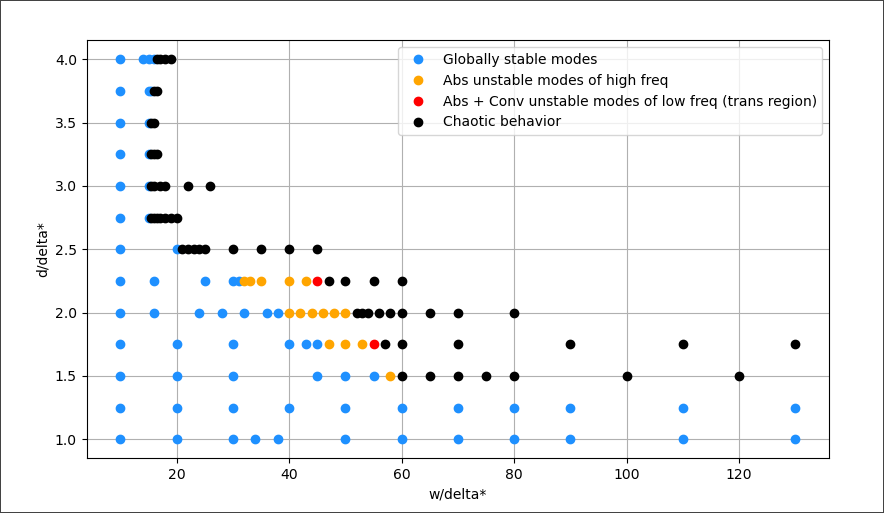
\includegraphics[width=0.98\linewidth]{Images/stabilitycurve.png}

			Check next slide to see figures (all representing the $v$ component of the velocity) in some cases.
		\end{column}
	\end{columns}

\end{frame}
\begin{frame}
	\centering
	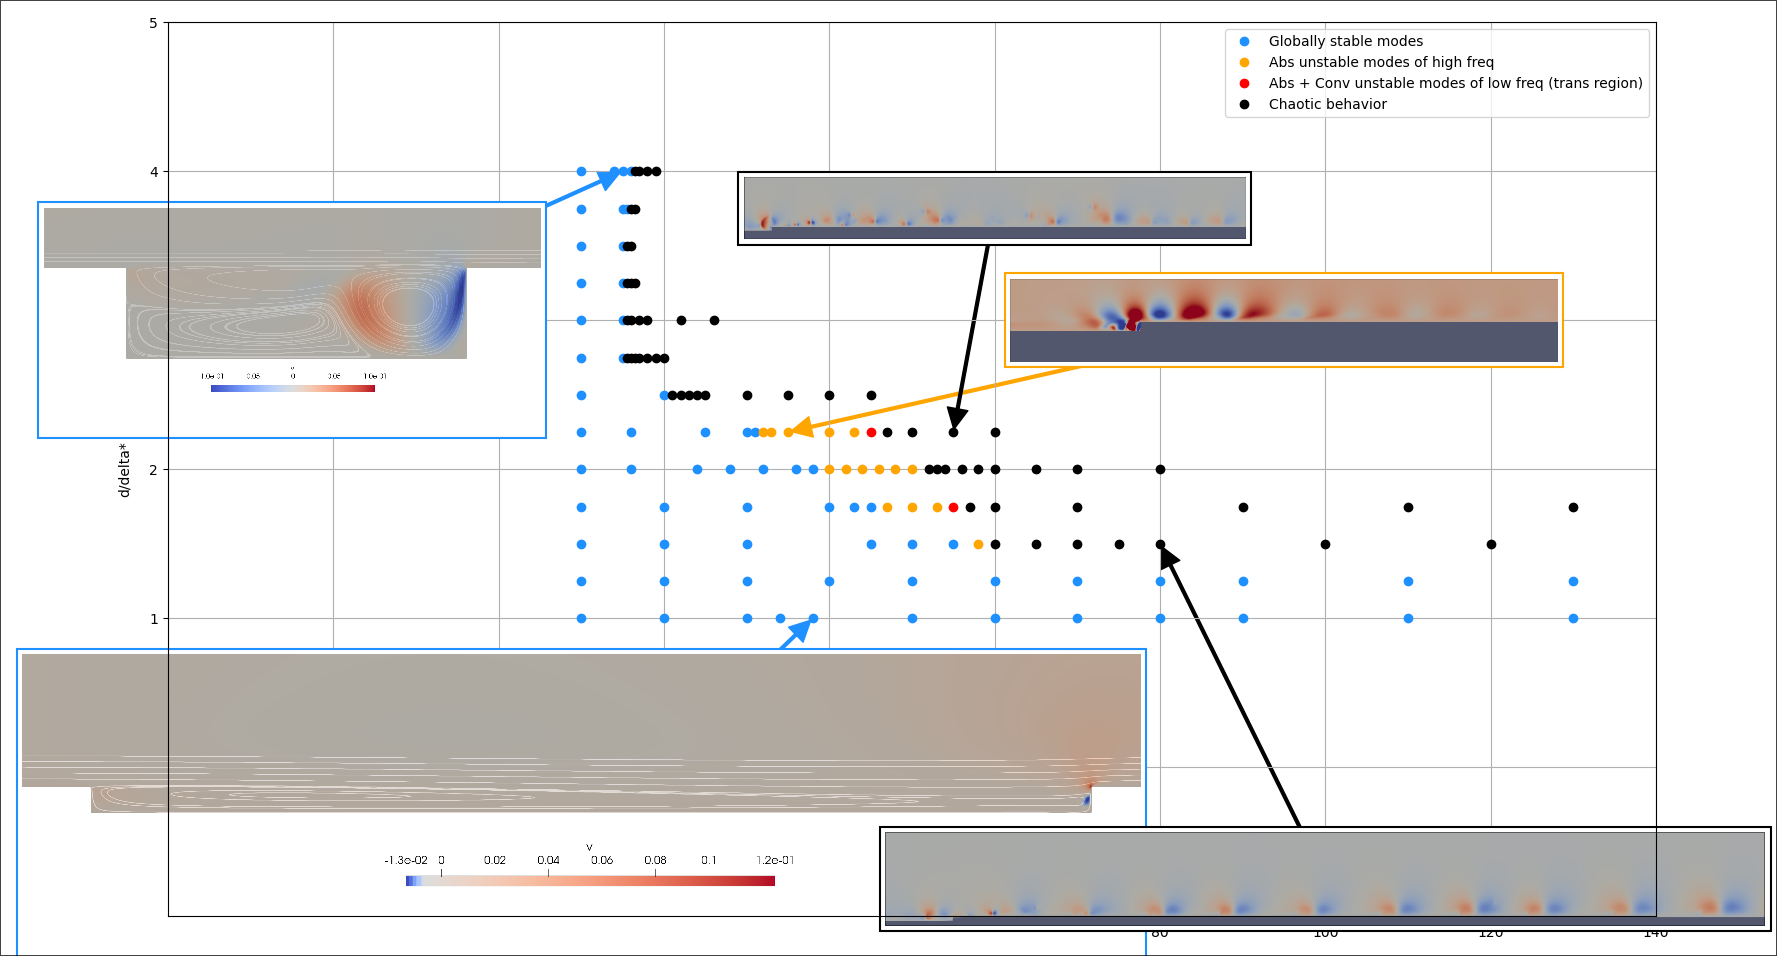
\includegraphics[width=0.98\linewidth]{Images/stabiliycurve_withImages.png}
\end{frame}
\begin{frame}
	\frametitle{Neutral curve for Blasius profile}
	\begin{itemize}
		\item This is orr-sommerfeld analysis for the Blasius profile and for different profiles (varying $x$ location) of the flat plate baseflow from DNS. They match pretty well.
		\item Increasing Reynolds = moving downstream in the domain.
		\item Neutral curve is for the growth rate of the TS mode, y-axis is the temporal frequency of the waves.
	\end{itemize}
	\centering
	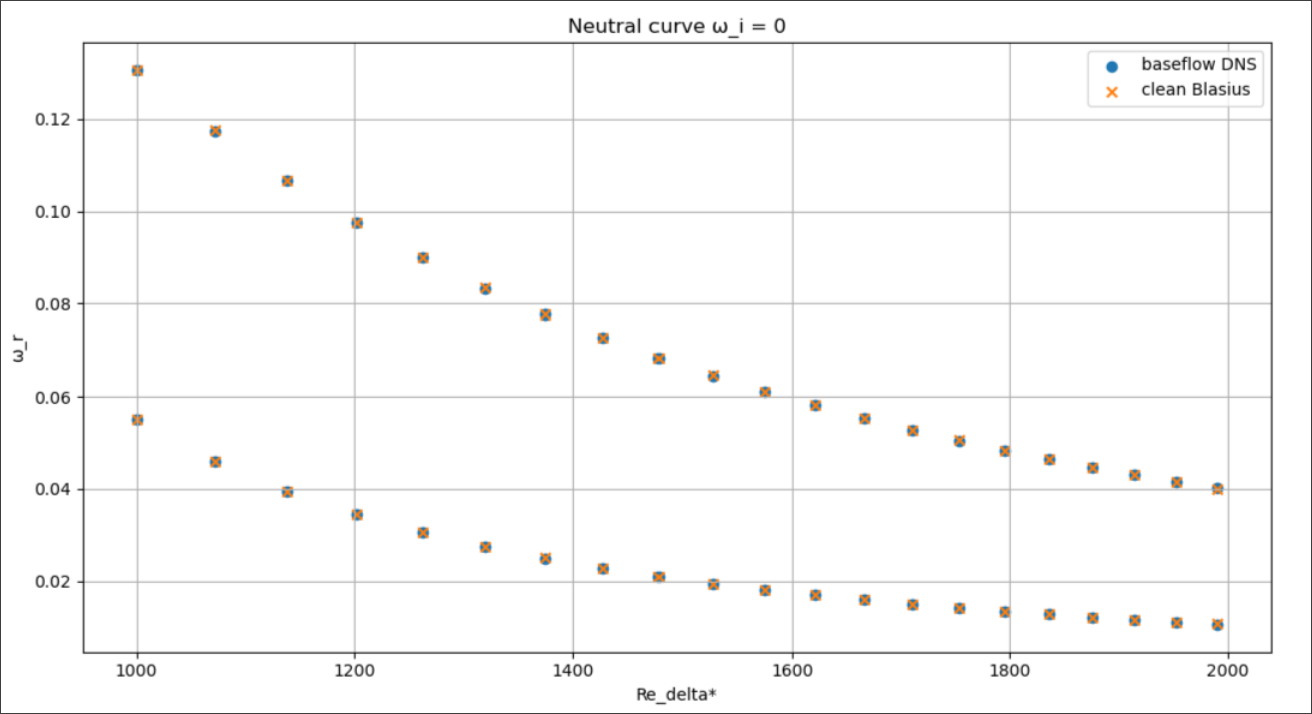
\includegraphics[width=0.7\linewidth]{Images/neutralcurve.png}
\end{frame}
\begin{frame}
	\frametitle{Ways to compute the n-factor}
	\begin{itemize}
		\item As we commented last time, we were unable to obtain the TS mode using our `default" EV finder (which founds the EVs with greatest real part). We tried another one, which should find the eigenvectors with eigenvalues closes to the origin, but it didn't work either (in this case, due to software problems, not physical ones).
		\item Then, we tried blowing and suction, which partially worked. By partially I mean that we were able to excite the TS mode, but they become damped at some point further downstream (see picture next slide).
		\item Now we started trying with transient growth in the flat-plate case and the results are promising.
	\end{itemize}

\end{frame}
\begin{frame}
	\begin{itemize}
		\item When blowing an suctioning at the same frequency
		      (green) there are times when the TS mode are damped
		      (bad). The ideal case would be to follow any of the purple curves (even more ideal, the centered one, corresponding to the most unstable frequency at any position), that is, getting the TS modes for a frequency inside the neutral curve and follow them downstream NATURALLY, as opposed to the blue curve.
	\end{itemize}
	\centering
	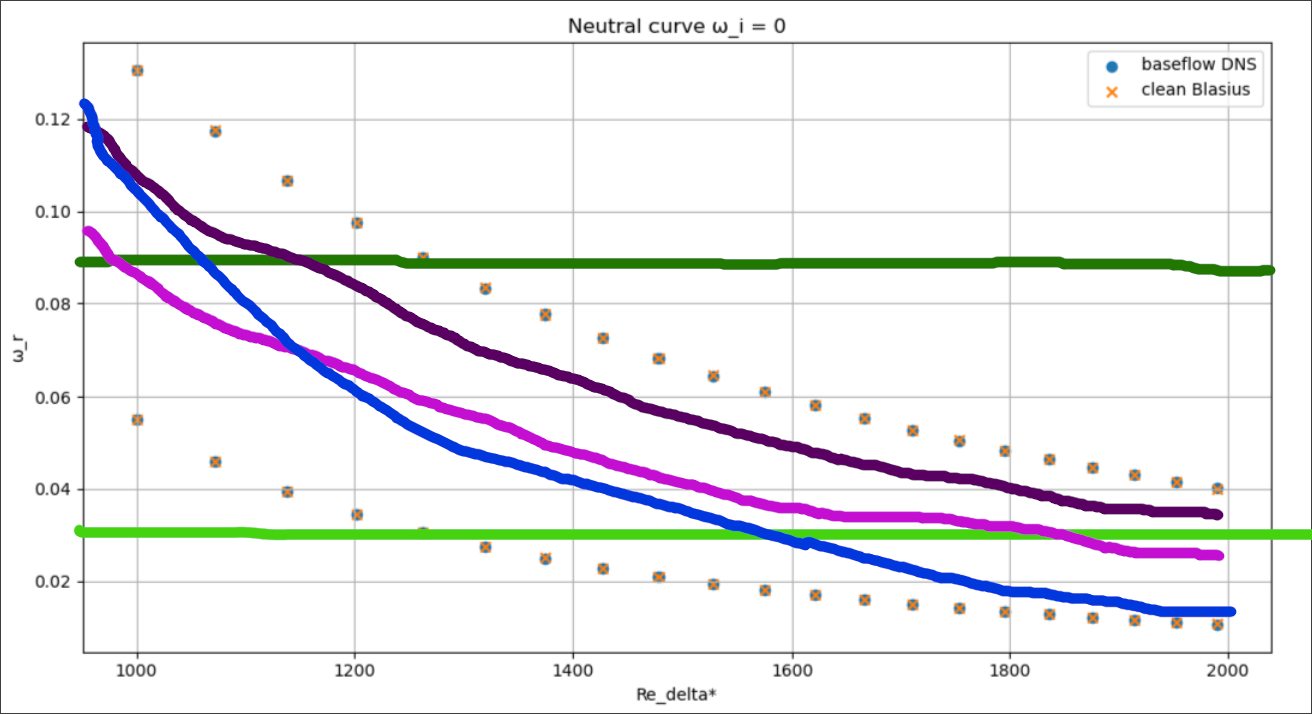
\includegraphics[width=0.75\linewidth]{Images/neutralcurve_wlines.png}

\end{frame}
\begin{frame}
	\frametitle{N-factor }
	\begin{itemize}
		\item The N-factor for several transient growth (TG) analysis.
		\item The result of TG is an the optimal initial condition giving the maximum energy at time $\tau$. Plot below shows TG for $\tau = 450,900, 1200$.
		\item Transient growth give us a wave packet that grows as it moves downstream (figure on the right).
	\end{itemize}
\begin{columns}[T] % [T] ensures correct vertical alignment
		\begin{column}{0.49\linewidth} % Left column
			\centering
			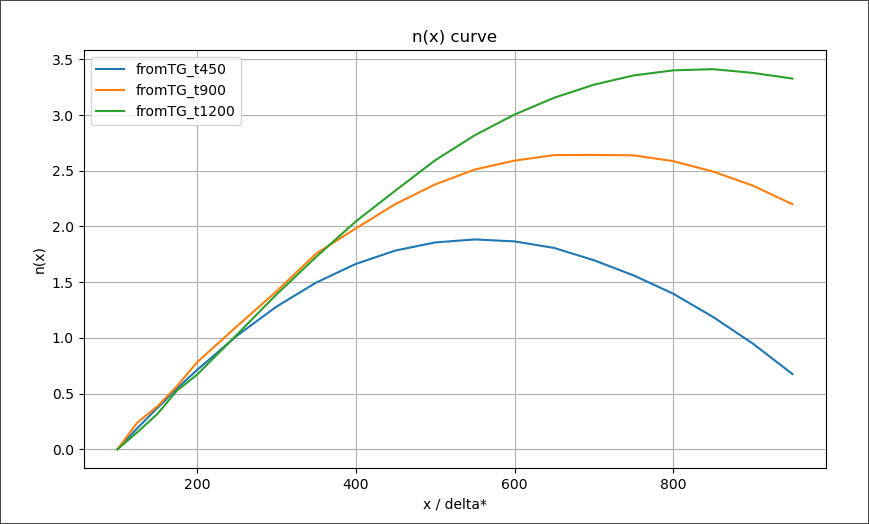
\includegraphics[width=0.98\linewidth]{Images/nfactorTG.png}
		\end{column}
		\begin{column}{0.49\linewidth} % Left column
			\centering
			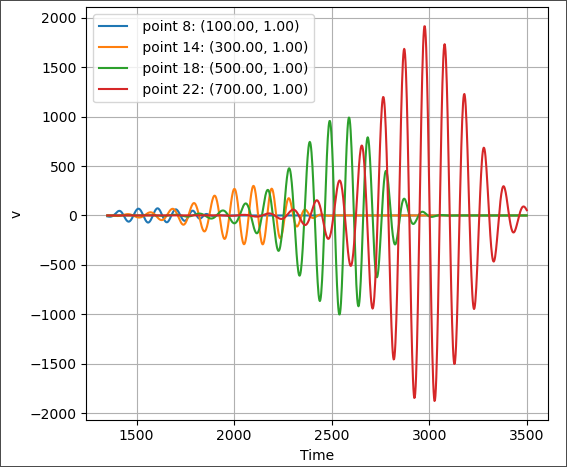
\includegraphics[width=0.98\linewidth]{Images/wavepacket.png}
		\end{column}
	\end{columns}

\end{frame}
\end{document}
